\begin{frame}[t]{Cài App Links cho một website}
  \SemLabel{MANIFEST · BỘ LỌC CỦA ACTIVITY ĐƯỢC EXPORT}\par\smallskip
  \noindent
  \begin{minipage}[t]{.755\linewidth}\vspace{0pt}
    \VerbatimInput[fontsize={\fontsize{7.9}{10.4}\selectfont},
      numbers=left,numbersep=4pt,xleftmargin=3.7mm]{snippets/app-link-filter-numbered.txt}
  \end{minipage}\hfill
  \begin{minipage}[t]{.225\linewidth}\vspace{0pt}\small\raggedright
    \SemLabel{1 · XÁC MINH}\par Kiểm tra host.\par\smallskip
    \SemLabel{2–4 · NHẬN LINK}\par VIEW và category.\par\smallskip
    \SemLabel{5–8 · PHẠM VI}\par Scheme, host, path.
  \end{minipage}\par
  \SemCallout{\textbf{TRÊN HOST HTTPS}\enspace\SemCode{https://example.org/.well-known/assetlinks.json}\par
    Thay host mẫu. Đăng tuyên bố khớp gói và chứng chỉ ký của APK.}
  \SemSource{\href{https://developer.android.com/training/app-links/add-applinks}{Khai báo bộ lọc} ·
    \href{https://developer.android.com/training/app-links/configure-assetlinks}{Cấu hình website}}
\end{frame}

\begin{frame}[t]{Đọc tuyên bố App Links của YouTube}
  \SemCallout{\SemLabel{HTTPS GET}\enspace\SemCode{www.youtube.com/.well-known/assetlinks.json}\hfill
    \textbf{200 · JSON}}
  \smallskip
  \noindent
  \begin{minipage}[t]{.62\linewidth}\vspace{0pt}
    \SemLabel{WEBSITE CÔNG BỐ · 3 DẤU VÂN TAY RÚT GỌN}
    \SemListingFile{snippets/youtube-dal-excerpt.txt}
  \end{minipage}\hfill
  \begin{minipage}[t]{.35\linewidth}\vspace{0pt}
    \SemBlueCard{Đo trên thiết bị}{%
      Host có \SemCode{verified}?\par
      Dấu vân tay khớp?\par
      Lần bấm mở app hay web?}
  \end{minipage}\par\smallskip
  \SemSource{25/11/2026 UTC · \href{https://www.youtube.com/.well-known/assetlinks.json}{Tệp công khai YouTube}
    · \href{https://developer.android.com/training/app-links/verify-applinks}{Cách đối chiếu trên thiết bị}}
\end{frame}

\begin{frame}[t]{UIT Mobile chuyển từ widget đến đúng ngày}
  \SemLead{Theo dõi một ngày từ dòng buổi học đến ô được chọn trong lịch.}
  \noindent\makebox[\linewidth][c]{%
    \begin{tikzpicture}[x=1mm,y=1mm,
      sem action/.style={-{Stealth[length=1.7mm]},Action,line width=.7pt},
      sem stage/.style={draw=Rule,fill=Paper,line width=.5pt,rounded corners=1mm}]
      \path[sem stage] (1,0) rectangle (42.5,28);
      \path[sem stage] (50,0) rectangle (91.5,28);
      \path[sem stage] (99,0) rectangle (140.5,28);
      \node[anchor=west] at (3,22) {\SemLabel{WIDGET · HÔM NAY}};
      \node[anchor=west] at (3,15) {\textbf{Dòng buổi học}};
      \node[anchor=west,fill=Ice,rounded corners=1mm] at (4,6) {\SemCode{25/11/2026}};
      \node[anchor=west] at (52,22) {\SemLabel{PENDINGINTENT}};
      \node[anchor=west] at (52,15) {\SemCode{MainActivity}};
      \node[anchor=west,fill=Ice,rounded corners=1mm] at (53,6) {\SemCode{date=2026-11-25}};
      \node[anchor=west] at (101,22) {\SemLabel{TAB LỊCH HỌC}};
      \node[anchor=west] at (101,15) {\textbf{Tháng 11/2026}};
      \foreach \day [count=\idx from 0] in {23,24,25,26,27,28,29} {
        \pgfmathsetmacro{\cellx}{104.1+\idx*5.15}
        \ifnum\day=25
          \node[fill=Navy,text=white,rounded corners=.8mm,inner sep=1.3mm] at (\cellx,6) {\scriptsize\bfseries \day};
        \else
          \node[text=Slate,inner sep=0pt] at (\cellx,6) {\scriptsize \day};
        \fi
      }
      \draw[sem action] (43.4,14) -- (49,14);
      \draw[sem action] (92.4,14) -- (98,14);
    \end{tikzpicture}}\par\medskip
  \SemCallout{\SemCode{uit-mobile://widget/schedule?date=}{\color{Action}\SemCode{2026-11-25}}}
  \smallskip
  Sơ đồ ngày minh họa. \SemCode{MainActivity} là nơi nhận, \SemCode{date} là ngày cần hiển thị.
  \SemSource{\href{https://developer.android.com/develop/ui/views/appwidgets/advanced}{Android App Widgets}
    · \href{https://developer.android.com/reference/android/app/PendingIntent}{PendingIntent}}
\end{frame}

\begin{frame}[t]{Widget gắn một Intent vào dòng buổi học}
  \noindent
  \begin{minipage}[t]{.645\linewidth}\vspace{0pt}
    \renewcommand{\SemListingFont}{\fontsize{8.5}{10.5}\selectfont}
    \SemLabel{Gắn vào dòng · ScheduleWidgetRenderer.kt}
    \SemListingFile{snippets/widget-bind.kt.txt}
    \SemLabel{Tạo thao tác mở · WidgetRoute.kt}
    \SemListingFile{snippets/widget-pending.kt.txt}
  \end{minipage}\hfill
  \begin{minipage}[t]{.323\linewidth}\vspace{0pt}
    \SemBlueCard{Intent đã chuẩn bị}{%
      \small \SemCode{MainActivity}\par
      \SemCode{ACTION_VIEW}\par
      \SemCode{date=2026-11-25}}
    \smallskip
    \SemCard{Khi chạm}{%
      \small Launcher kích hoạt thao tác đã gắn. \SemCode{IMMUTABLE} giữ URI khỏi bị sửa lúc gửi.}
  \end{minipage}\par
  \SemSource{\href{https://developer.android.com/reference/android/widget/RemoteViews\#setOnClickPendingIntent(int,android.app.PendingIntent)}{RemoteViews}
    · \href{https://developer.android.com/reference/android/app/PendingIntent}{PendingIntent}}
\end{frame}

\begin{frame}[t]{Activity nhận link ở hai thời điểm}
  \noindent\makebox[\linewidth][c]{%
    \begin{tikzpicture}[x=1mm,y=1mm,
      sem lifecycle/.style={draw=Rule,fill=Paper,rounded corners=1mm,minimum height=14mm,text width=56mm,align=center},
      sem lifecycle arrow/.style={-{Stealth[length=1.7mm]},Action,line width=.65pt}]
      \node[sem lifecycle] (cold) at (32,27) {\SemLabel{TẠO ACTIVITY MỚI}\\\SemCode{onCreate()}};
      \node[sem lifecycle] (warm) at (108,27) {\SemLabel{TÁI SỬ DỤNG ACTIVITY}\\\SemCode{onNewIntent()}};
      \node[sem lifecycle,fill=Navy,draw=Navy,text=white,text width=48mm,minimum height=9mm] (route) at (70,4) {\SemCode{WidgetRoute.read(...)}};
      \draw[sem lifecycle arrow] (cold.south) -- ++(0,-7) -| ([xshift=-14mm]route.north);
      \draw[sem lifecycle arrow] (warm.south) -- ++(0,-7) -| ([xshift=14mm]route.north);
    \end{tikzpicture}}\par\medskip
  \SemLabel{Nhánh tái sử dụng · MainActivity.kt}
  \SemListingFile{snippets/widget-new-intent.kt.txt}
  \SemCode{singleTop} cho phép Activity trên cùng nhận Intent mới.\par
  Nếu chỉ đọc ở \SemCode{onCreate()}, lần gửi tiếp có thể giữ ngày cũ.
  \SemSource{\href{https://developer.android.com/guide/components/activities/tasks-and-back-stack}{Activity, task và back stack}}
\end{frame}

\begin{frame}[t]{Router biến ngày trong URI thành giao diện}
  \noindent
  \begin{minipage}[t]{.68\linewidth}\vspace{0pt}
    \renewcommand{\SemListingFont}{\fontsize{8.5}{10.5}\selectfont}
    \SemLabel{Kiểm tra ngày · WidgetRoute.kt}
    \SemListingFile{snippets/widget-date.kt.txt}
    \SemLabel{Đưa ngày vào lịch · MainActivity.kt}
    \SemListingFile{snippets/widget-focus.kt.txt}
  \end{minipage}\hfill
  \begin{minipage}[t]{.29\linewidth}\vspace{0pt}
    \SemLabel{BA KẾT QUẢ}\par\smallskip
    \SemCallout{\small
      \textbf{Ngày hợp lệ}\par Lịch chọn 25/11.\par\medskip
      \textbf{Thiếu \SemCode{date}}\par Dùng \SemCode{today()}.\par\medskip
      \textbf{Ngày không hợp lệ}\par Bỏ route.}
  \end{minipage}
\end{frame}

\begin{frame}[t]{Bấm widget trên điện thoại}
  \noindent
  \begin{minipage}[t]{.362\linewidth}\vspace{0pt}
    \SemLabel{BỘ CHỌN TRONG APP}\par\smallskip
    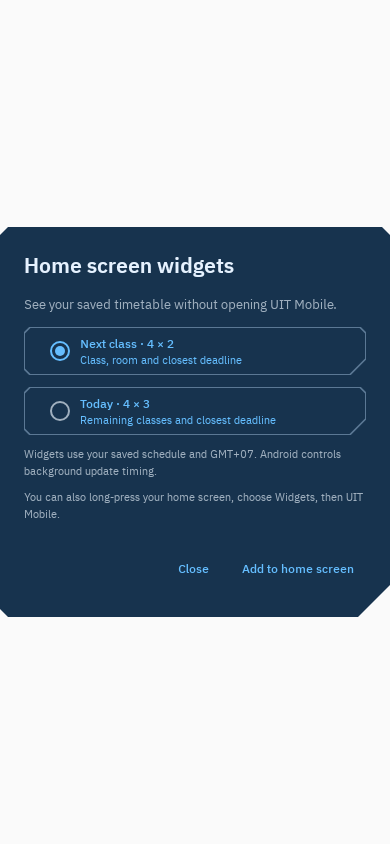
\includegraphics[width=.96\linewidth,trim=16bp 398bp 16bp 319bp,clip]{assets/demo/widget-picker-phone.png}\par\smallskip
    \SemLabel{WIDGET CHƯA LIÊN KẾT}\par\smallskip
    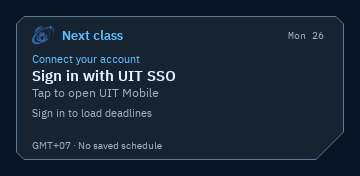
\includegraphics[width=.96\linewidth,trim=0bp 12bp 0bp 12bp,clip]{assets/demo/widget-signed-out-360.png}\par
    \SemSource{Ảnh render từ giao diện UIT Mobile}
  \end{minipage}\hfill
  \begin{minipage}[t]{.60\linewidth}\vspace{0pt}
    \begin{enumerate}
      \item Cài \SemCode{UIT-Mobile-SE114.apk}. Mở từ biểu tượng để quan sát màn hình đầu.
      \item Thêm \textbf{UIT Mobile · Hôm nay} trong bộ chọn Widget của Launcher.
      \item Chạm dòng buổi học đã lưu. So ngày trên dòng đó với ngày được chọn trong \textbf{Lịch học}.
    \end{enumerate}
    \smallskip
    \textbf{Chưa liên kết:} chạm thẻ sẽ mở Hồ sơ.
  \end{minipage}
\end{frame}

\begin{frame}[t]{Đổi ngày trong URI bằng ADB}
  \SemLead{Đổi \SemCode{date} từ 25/11 sang 26/11 và quan sát ngày được chọn.}
  \SemListingFile{snippets/widget-adb.txt}
  \noindent
  \begin{minipage}[c]{.358\linewidth}
    \SemLabel{TẠO ACTIVITY · 25/11}\par\smallskip
    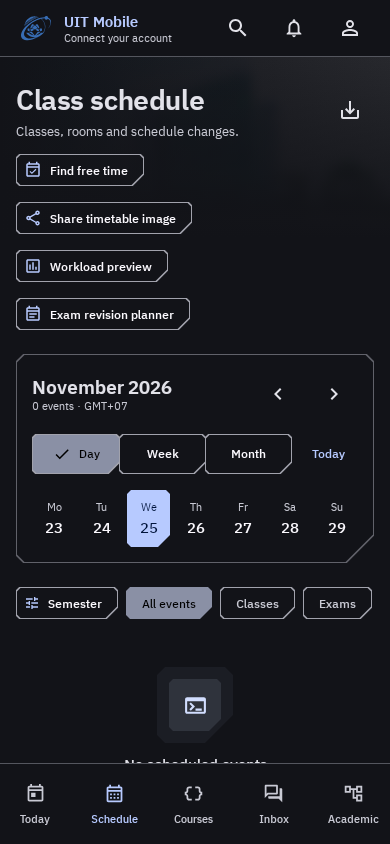
\includegraphics[width=\linewidth,trim=12bp 278bp 12bp 352bp,clip]{assets/demo/schedule-empty-2026-11-25.png}\par
  \end{minipage}\hfill
  \begin{minipage}[c]{.19\linewidth}
    \centering
    \SemLabel{GIỮ ACTIVITY}\par
    Đổi \SemCode{date}\par
    {\color{Action}\(\longrightarrow\)}\par
  \end{minipage}\hfill
  \begin{minipage}[c]{.358\linewidth}
    \SemLabel{NHẬN INTENT MỚI · 26/11}\par\smallskip
    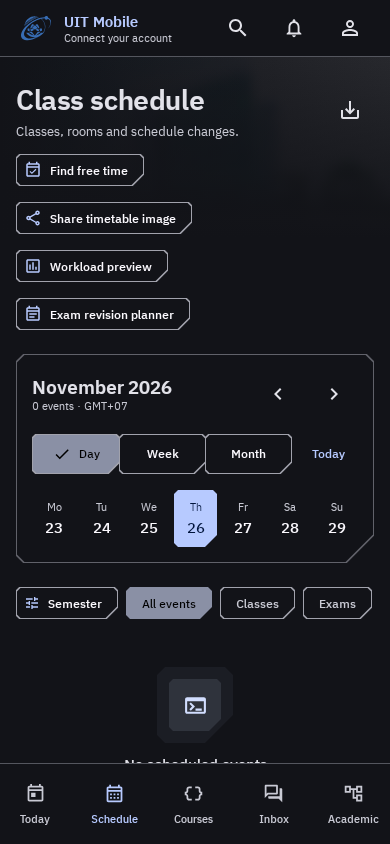
\includegraphics[width=\linewidth,trim=12bp 278bp 12bp 352bp,clip]{assets/demo/schedule-empty-2026-11-26.png}\par
  \end{minipage}\par
  \SemSource{Robolectric · Lịch UIT Mobile với dữ liệu trống · \href{https://developer.android.com/tools/adb}{ADB} dùng \SemCode{-n} chỉ Activity, \SemCode{-d} truyền URI.}
\end{frame}

\begin{frame}[t]{Đúng ứng dụng, đúng nội dung}
  \SemLead{Hai cách chọn bên nhận. Cùng một việc sau khi nhận URI.}
  \noindent\makebox[\linewidth][c]{%
    \begin{tikzpicture}[x=1mm,y=1mm,
      sem summary/.style={draw=Rule,fill=Paper,rounded corners=1mm,text width=43mm,align=center,inner sep=2mm,minimum height=14mm},
      sem summary arrow/.style={-{Stealth[length=1.7mm]},Action,line width=.65pt}]
      \node[sem summary] (web) at (26,27) {\SemLabel{URL HTTPS}\\Android phân giải};
      \node[sem summary] (widget) at (26,8) {\SemLabel{WIDGET}\\Activity đã được chỉ định};
      \node[sem summary,text width=30mm] (activity) at (82,17.5) {\textbf{Activity}\\Nhận URI};
      \node[sem summary,fill=Navy,draw=Navy,text=white,text width=30mm] (destination) at (123,17.5) {\textbf{Nội dung}\\Đọc và mở đích};
      \draw[sem summary arrow] (web.east) -- ++(7,0) |- ([yshift=2mm]activity.west);
      \draw[sem summary arrow] (widget.east) -- ++(7,0) |- ([yshift=-2mm]activity.west);
      \draw[sem summary arrow] (activity.east) -- (destination.west);
    \end{tikzpicture}}\par\medskip
  \SemCallout{\textbf{Hỏi đáp.} App đã mở, lịch vẫn ở sai ngày. Bạn kiểm tra URI, bộ đọc hay giao diện trước?}
\end{frame}
